%==============================================================================
%== template for LATEX poster =================================================
%==============================================================================
%
%--A0 beamer slide-------------------------------------------------------------
\documentclass[final]{beamer} % use beamer
\usepackage[orientation=portrait,
            size=a0,          % poster size
            scale=1.1         % font scale factor
           ]{beamerposter}    % beamer in poster size
%
%--some needed packages--------------------------------------------------------
\usepackage[american]{babel}  % language 
\usepackage[utf8]{inputenc}   % std linux encoding
\usepackage{caption}
\usepackage{subcaption}
% \usepackage[11pt]{moresize}
%
%==The poster style============================================================
\usetheme{cpbgposter}            % our poster style
%--set colors for blocks (without frame)---------------------------------------
  \setbeamercolor{block title}{fg=ngreen,bg=white}
  \setbeamercolor{block body}{fg=black,bg=white}
%--set colors for alerted blocks (with frame)----------------------------------
%--textcolor = fg, backgroundcolor = bg, dblue is the jacobs blue
  \setbeamercolor{block alerted title}{fg=white,bg=dblue!70}%frame color
  \setbeamercolor{block alerted body}{fg=black,bg=dblue!10}%body color
%
%==Titel, date and authors of the poster=======================================
\title{Finger formation at the base of ash clouds: \\ A linear stability analysis}
\author[shortname]{Paul Jarvis \inst{1} \and Jonathon Lemus \inst{1} \and
  Allan Fries \inst{1} \\ \and Amanda Clarke \inst{2} \and Jeremy Phillips \inst{3}
  \and Costanza Bonadonna \inst{1}}
\institute[shortinst]{\inst{1} Section of Earth and Environmental Sciences,
  University of Geneva \and
  \inst{2} School of Earth and Space Exploration, Arizona State University \and
  \inst{3} School of Earth Sciences, University of Bristol}

%
%==some usefull fluit dynamics====================================================
\newcommand\Rey{\mbox{\textit{Re}}}  % Reynolds number
%==============================================================================
%==the poster content==========================================================
%==============================================================================
\begin{document}
%--the poster is one beamer frame, so we have to start with:
\begin{frame}[t]

  \begin{columns}[t]

    \begin{column}{0.6\paperwidth}

      \begin{columns}[t]

        \begin{column}{0.3\paperwidth}
          \begin{figure}
            \includegraphics[width=\textwidth]{Sabancaya_fingers.png}
          \end{figure}

          \centering \footnotesize Figure 1. a) Visible and b) infrared images of
          ash clouds from Vulcanian explosions of Sabancaya volcano, Peru. Fingers
          can be seen in both images.

        \end{column}

        \begin{column}{0.3\paperwidth}
          \begin{block}{Introduction}
            \centering Volcanic ash presents a hazard for infrastructure and human
            health. Understanding ash settling is therefore crucial for assessing
            the associated risk. Downard-propagating fingers(Figure 1), hypothesised
            to form from a gravitational instability at the base of the ash cloud
            (Figure 2) have been seen at many volcanoes. Here we present a linear
            stability analysis, that predicits the initial growth rate of the
            fingers. 
          \end{block}

        \end{column}
      \end{columns}

      \begin{block}{Equations of motion}

        \begin{columns}[t]

          \begin{column}{0.3\paperwidth}
            $$ \mathbf{\nabla} \cdot \mathbf{u}(\mathbf{x}, t) $$

            $$ \frac{\partial \mathbf{u}(\mathbf{x}, t)}{\partial t} +
            [\mathbf{u}(\mathbf{x}, t)] \cdot \mathbf{\nabla}]
              \mathbf{u}(\mathbf{x}, t) =
              \frac{\mathbf{\nabla} P(\mathbf{x}, t)}{\rho_{0}} +
              \nu \nabla^{2} \mathbf{u}(\mathbf{x}, t) - g'\mathbf{\hat{z}} $$

              $$ \frac{\partial \phi(\mathbf{x}, t)}{\partial t} +
              [\mathbf{u}(\mathbf{x}, t)] - \mathbf{U_{\text{p}}}] \cdot
                \mathbf{\nabla} \phi(\mathbf{x}, t) =
                D_{\text{p}} \nabla^{2} \phi(\mathbf{x}, t) $$

                $$ \frac{\partial s(\mathbf{x}, t)}{\partial t} +
                \mathbf{u}(\mathbf{x}, t)x \cdot \mathbf{\nabla} s(\mathbf{x}, t) =
                D_{\text{s}} \nabla^{2} s(\mathbf{x}, t) $$

                $$ g' = g \left( [1 + \alpha s(\mathbf{x}, t)] [1 - \phi(\mathbf{x}, t)]
                + \frac{\rho_{p} \phi(\mathbf{x}, t)}{\rho_{0}} \right) $$

          \end{column}

          \begin{column}{0.07\paperwidth}

            \centering

            \vspace{-0.5cm}

            Conservation of \\ mass \\

            \vspace{0.7cm}

            Conservation of \\ momentum \\

            \vspace{0.7cm}

            Conservation of \\ particles \\

            \vspace{0.7cm}

            Conservation of \\ solute \\

            \vspace{0.7cm}

            Reduced gravity \\

          \end{column}

          \begin{column}{0.23\paperwidth}

            \vspace{2cm}

            \begin{tabular}{| c | l | c | l |}
              \hline
              \multicolumn{2}{ | c |}{\textbf{Unknowns}}             & \multicolumn{2}{| c |}{\textbf{Parameters}}\\
              \hline
              $\mathbf{u}(\mathbf{x}, t)$ & Fluid velocity           & $\rho_{0} $           & Reference fluid density \\
              $P(\mathbf{x}, t)$          & Pressure                 & $\nu$                & Kinematic viscosity \\
              $\phi(\mathbf{x}, t)$       & Particle volume          &$\mathbf{U_{\text{p}}}$ & Particle settling velocity \\
              $s(\mathbf{x}, t)$          & Solute concentration     & $\rho_{\text{p}}$      & Particle density \\
              \cline{1-2}
              \multicolumn{2}{ | c |}{\textbf{Variables}}            & $D_{\text{p}}$         & Particle diffusivity \\
              \cline{1-2}
              $\mathbf{x}$                & Position vector          & $D_{\text{s}}$         & Solute diffusivity \\
              $t$                         & time                     & $g$                  & Gravity \\
              $\mathbf{\hat{z}}$          & Vertical unit vector     & $\alpha$             & Expansivity \\
              \hline  
            \end{tabular}      
      
          \end{column}

        \end{columns}
      \end{block}
      
    \end{column}

    \begin{column}{0.3\paperwidth}

      \vspace{-3cm}
      
      \begin{columns}[t]
        \begin{column}{0.12\paperwidth}

          \vspace{-2.2cm}

          \begin{figure}
            \includegraphics[height=20cm]{init_config.pdf}
          \end{figure}
        \end{column}

        \begin{column}{0.17\paperwidth}
          
          \begin{figure}
            \includegraphics[height=18cm]{unstable_config.pdf}
          \end{figure}
        \end{column}
        
      \end{columns}

      \vspace{-1cm}

      \centering \footnotesize Figure 2. Despite an initial stable
      configuration, ash settling leads to the formation of a gravitationally
      unstable \textbf{particle boundary layer}.

      \vspace{1cm}

      
    \end{column}
    
  \end{columns}


  \begin{columns}[t]
    \begin{column}{0.3\paperwidth}
      \begin{block}{Expansion: Base state + Perturbation}
        $$ \mathbf{u}(\mathbf{x}, t) = \mathbf{u}^{(0)}(\mathbf{x}, t) +
        \mathbf{\hat{u}}(z) e^{i(k_{x} x + k_{y} y - \omega t)},
        \quad \mathbf{\hat{u}} \ll \mathbf{u}^{(0)} $$

        $$ P(\mathbf{x}, t) = P^{(0)}(\mathbf{x}, t) +
        \hat{P}(z) e^{i(k_{x} x + k_{y} y - \omega t)},
        \quad \hat{P} \ll P^{(0)} $$

        $$ \phi(\mathbf{x}, t) = \phi^{(0)}(\mathbf{x}, t) +
        \hat{\phi}(z) e^{i(k_{x} x + k_{y} y - \omega t)},
        \quad \hat{\phi} \ll \phi^{(0)}  $$
      
        $$ s(\mathbf{x}, t) = s^{(0)}(\mathbf{x}, t) +
        \hat{s}(z) e^{i(k_{x} x + k_{y} y - \omega t)},
        \quad \hat{s} \ll s^{(0)}  $$
      \end{block}

    \end{column}

    \begin{column}{0.6\paperwidth}

%      $$ \frac{1}{\Rey} \frac{\mathrm{d}^{4} \hat{u_{z}}}{\mathrm{d} z'} - u_{z}^{0} \frac{\mathrm{d}^{3} \hat{u_{z}}}{\mathrm{d} z'^{3}} - \left(\frac{2 k^{2}}{\Rey} + \frac{\partial u_{z}^{0}}{\partial z'} + i k_{x} u_{x}^{0} \right) \frac{\mathrm{d}^{2} \hat{u_{z}}}{\mathrm{d} z'^{2}} + \left(k^{2} u_{z}^{0} - i k_{x} \frac{\partial u_{x}^{0}}{\partial z'} \right) \frac{\mathrm{d} \hat{u_{z}}}{\mathrm{d} z'} + \left[k^{2} \left(\frac{k^{2}}{\Rey} + i k_{x} u_{x}^{0}\right) + i k_{x} \frac{\partial^{2} u_{x}^{0}}{\partial z'^{2}}\right] \hat{u_{z}} + k^{2} A_{\beta} (1 - \phi^{0}) \hat{s} + k^{2} (A_{\gamma} - A_{\beta} s^{0}) \hat{\phi} = -i \omega \left(\frac{\mathrm{d}^{2} \hat{u_{z}}}{\mathrm{d} z'^{2}} - k^{2} \hat{u_{z}}\right)$$

    \end{column}

  \end{columns}


      
%    \begin{column}{0.3\paperwidth}
%      \begin{block}{Perturbations}
%
%      \end{block}
%
%
%    \end{column}
    

      
\end{frame}
\end{document}
